% Created 2016-11-04 Fr 11:40
\documentclass[11pt]{article}
\usepackage[utf8]{inputenc}
\usepackage[T1]{fontenc}
\usepackage{fixltx2e}
\usepackage{graphicx}
\usepackage{longtable}
\usepackage{float}
\usepackage{wrapfig}
\usepackage{rotating}
\usepackage[normalem]{ulem}
\usepackage{amsmath}
\usepackage{textcomp}
\usepackage{marvosym}
\usepackage{wasysym}
\usepackage{amssymb}
\usepackage{hyperref}
\tolerance=1000
\usepackage{siunitx}
\usepackage{fontspec}
\sisetup{load-configurations = abbrevations}
\newcommand{\estimates}{\overset{\scriptscriptstyle\wedge}{=}}
\usepackage{mathtools}
\DeclarePairedDelimiter\abs{\lvert}{\rvert}%
\DeclarePairedDelimiter\norm{\lVert}{\rVert}%
\makeatletter
\let\oldabs\abs
\def\abs{\@ifstar{\oldabs}{\oldabs*}}
\let\oldnorm\norm
\def\norm{\@ifstar{\oldnorm}{\oldnorm*}}
\makeatother
\DeclareMathOperator{\Exists}{\exists}
\DeclareMathOperator{\Forall}{\forall}
\def\cvec#1{\left(\vcenter{\halign{\hfil$##$\hfil\cr \cvecA#1;;}}\right)}
\def\cvecA#1;{\if;#1;\else #1\cr \expandafter \cvecA \fi}
\renewcommand{\d}{\mathrm{d}}
\newcommand{\f}[2]{\frac{#1}{#2}}
\renewcommand{\v}[1]{\vec{#1}}
\usepackage{pgfplots}
\author{Robin Heinemann}
\date{\today}
\title{Theoretische Physik (Hebecker)}
\hypersetup{
  pdfkeywords={},
  pdfsubject={},
  pdfcreator={Emacs 25.1.1 (Org mode 8.2.10)}}
\begin{document}

\maketitle
\tableofcontents

Einleitung: \\
\begin{itemize}
\item Webseite: www.thphys.uni-heidelberg.de/hebecker/TP1/tp1.html
\item Bartelman skripte
\end{itemize}

\section{Kinematik des Massenpunktes}
\label{sec-1}
Massenpunkt / Punktmasse - (selbstevidente) Abstraktion
Kinematik: Bescheibung der Bewegung (Ursachen der Bewegung $\rightarrow$ Dynamik)
\subsection{Kinematik der Massenpunktes in \underline{einer} Dimension}
\label{sec-1-1}
\subsubsection{Graphik}
\label{sec-1-1-1}
\begin{itemize}
\item Ort: $x$
\item zu Zeit $t:~x(t)$
\item Geschwindigketi: $v(t) \equiv \frac{\mathrm{d}x(t)}{\mathrm{d}t} \equiv \dot{x}(t)$
\item Beschleunigung: $a(t) \equiv \dot{v}(t) = \ddot{x}(t)$
\item Beispiel: $x(t) \equiv x_0 + v_0 t + \frac{a_0}{2},~t^2,~v(t) = v_0 + a_0 t,~a(t) = a_0$
\item Umgekehrt: Integration, z.B. von Geschwindigkeit zu Trajektorie: Anfangsposition muss gegeben sein, z.B. $x(t_0) \equiv x_0$
     \[x(T)=x_0 + \int_{t_0}^{t}v(t)\mathrm{d}t\]
     Man prüft leicht $\dot{x}(t) = v(t)$
\begin{itemize}
\item Es gibt keine andere Funktion $\tilde{x}(t)$ mit $\dot{\tilde{x}}(t) = v(t)$ und $\tilde{x}(t_0) = x_0$
\end{itemize}
Analog: Von Beschleunigung zur Geschwindigkeit, und dann weiter zur Trajektorie
\end{itemize}
\subsubsection{Üben dieser Logik an unserem Beispiel}
\label{sec-1-1-2}
Gegeben: $a(t) = a_0,~t_0=0,v_0,x_0$ \\
    \[\Rightarrow~v(t) = v_0 + \int_0^t a_0\mathrm{d}t' = v_0 + a_0 t\]
\[x(t) = x_0 + \int_0^t (v_0 + a_0 t')\mathrm{d}t' = x_0 + v_0 t + \frac{a_0}{2}t^2\]
\subsection{Grundbegriffe der Differenzial und Integralrechung}
\label{sec-1-2}
\subsubsection{Funktion}
\label{sec-1-2-1}
\[f: \mathbb{R} \rightarrow \mathbb{R},~x \mapsto f(x)\]
\subsubsection{Differentiation oder Ableitung}
\label{sec-1-2-2}
\[\frac{\mathrm{d}f(x)}{\mathrm{d}x} = f'(x) = \lim_{\Delta x \to 0} \frac{f(x + \Delta x) - f(x)}{\Delta x}\]
$\mathrm{d}f$ bezeichnet den in $\Delta x$ linearen Anteil des Zuwaches $\Delta f\equiv f(x + \Delta x) - f(x)$.
\begin{itemize}
\item Aus $\Delta f = f'(x)\Delta(x) + O(\Delta x^2)~\text{folgt}~\mathrm{d}f = f'(x)\Delta x$
\item Anwendung auf die Identitätabbildung: $x \mapsto x \Rightarrow \mathrm{d}x = \Delta x$
      \[\Rightarrow \mathrm{d}f = f'(x)\mathrm{d}x~\text{oder}~\frac{\mathrm{d}f(x)}{\mathrm{d}x} = f'(x)\]
      Dies ist eigentlich nur eine Schreibweise für $f'(x)$, \uline{aber} nützlich, weil bei kleinen $\Delta x~\mathrm{d}f \simeq \Delta f$ (Schreibweise beinhaltet intuitiv die Grenzwertdefinition)
\item $f'(x)$ wieder Funktion $\Rightarrow$ analog: $f''(x),~f'''(x),\ldots,f^{(n)}(x)$
\item Praxis
\[(f\cdot g)' = f' g + g' f~\text{(Produkt/Leibnizregel)}\]
\[(f \circ g)'(x) = f'(g(x))g'(x)~\text{(Kettenregel)}\]
\[(f^{-1})'(x) = \frac{1}{f'(f^{-1}(x))}~\text{(Ableitung der Inversen Funktion)}\]
\begin{itemize}
\item Begründung (nur zum letzen Punkt)
\[(f^{-1})'(x) = \frac{\mathrm{d}y}{\mathrm{d}x} = \frac{\mathrm{d}y}{\mathrm{d}(f(y))} = \frac{\mathrm{d}y}{f'(y)\mathrm{d}y} = \frac{1}{f'(f^{-1}(x))}\]
\item Schöne Beispiele
\[(x^x)' = (e^{\ln{x^x}})' = (e^{x\ln{x}})' = e^{x\ln{x}}(\ln{x} + 1) = x^x(\ln{x} + 1)\]
\[\arctan'(x) \equiv (\tan^{-1}(x)) = \frac{1}{\tan^{-1}(y)}~\text{wobei $y = \tan^{-1}(x)$}\]
Besser: \[\tan^{-1}(y) = (\sin{y} \frac{1}{\cos{y}})' = \cos{y} \frac{1}{\cos{y}} + \sin{y}(\frac{1}{\cos{y}})' = 1 + \sin{y}(-\frac{1}{\cos^2{y}})(-\sin{y}) = 1 + \tan^2{y} = 1 + x^2 \\ \Rightarrow \arctan'(x) = \frac{1}{1 + x^2}\]
\end{itemize}
\item Verknüpfung \[f\circ g: x\mapsto f(g(x))\]
\item Inverse \[f^{-1} : x=f(y)\mapsto y\]
\item Grenzwerte:
\begin{itemize}
\item nützliche Regel: l'Hôpital ("$\frac{0}{0}$") \\
        Falls $\lim_{x\to x_0} f,g = 0$ und $\lim_{x\to x_0} \frac{f'}{g'}$ existiert, so gilt $\lim_{x\to x_0}\frac{f}{g} = \lim_{x\to x_0} \frac{f'}{g'}$
\item weitere nützliche Regel \[\lim \frac{\text{Beschränkt}}{\text{Unbeschränkt und monoton wachsend}} = 0\]
\begin{itemize}
\item Beispiel: \[\lim_{y\to 0} \frac{\sin{\frac{1}{y}}}{\frac{1}{y}}\]
\end{itemize}
\item Kürzen unter $\lim$
\begin{itemize}
\item Beispiel: \[\lim_{x\to\infty} \frac{x}{2x + \sqrt{x}} = \lim_{x\to\infty}\frac{1}{2+\frac{1}{\sqrt{x}}} = \frac{1}{2}\]
\end{itemize}
\end{itemize}
\end{itemize}
\subsubsection{Integrieren}
\label{sec-1-2-3}
\begin{enumerate}
\item Fundamentalsatz der Analysis
\label{sec-1-2-3-1}
\[\int^y f(x)\mathrm{d}x = F(y) \& F'(y) = f(y)\]
\[\int f(x)\mathrm{d}x = F(x) + C\]
\[\int_a^b f(x)\mathrm{d}x = F(b) - F(a)\]
($\to$ saubere Definition über Riemansches Integral)
\item Praxis
\label{sec-1-2-3-2}
\begin{enumerate}
\item Partielle Integration
\label{sec-1-2-3-2-1}
\[\int^y f(x)g'(x)\mathrm{d}x = f(y)g(y) - \int^y f'(x)g(x)\mathrm{d}x\]
\item Substitution
\label{sec-1-2-3-2-2}
Unter Annahme einer invertierbaren Funktion $x: y\mapsto x(y)$
\[\int f(x)\mathrm{d}x = \int f(x)\frac{\mathrm{d}x}{\mathrm{d}y}\mathrm{d}y = \int f(x(y)) x'(y)\mathrm{d}y\]
Andere Formulierung: \[\int_a^b f(g(x))g'(x)\mathrm{d}x = \int_{g(a)}^{g(b)}f(y)\mathrm{d}y\]
Substitution $y=g(x)$
\item Klassiker
\label{sec-1-2-3-2-3}
\[\int \ln{x}\mathrm{d}x = \int \ln{x}1\mathrm{d}x = \ln{x}x - \int \frac{1}{x}x\mathrm{d}x = x(\ln{x} - 1)\]
\[\int x e^{x^2}\mathrm{d}x = \int e^{x^2}\frac{1}{2}\mathrm{d}(x^2) = \frac{1}{2}\int e^y \mathrm{d}y = \frac{1}{2}e^y = \frac{1}{2}e^{x^2}\]
\end{enumerate}
\end{enumerate}
\subsection{Kinematik in mehreren Dimensionen}
\label{sec-1-3}
\subsubsection{Zweidimensionale Bewegung}
\label{sec-1-3-1}
Zweidimensional $\rightarrow$ Bewegung in der Ebene. Trajektorie: $x(t),y(t)$
\begin{enumerate}
\item Bespiel
\label{sec-1-3-1-1}
\[x(t) = v_0 t \sin{\omega t}\]
\[y(t) = v_0 t \cos{\omega t}\]
\begin{enumerate}
\item {\bfseries\sffamily TODO} Skizze der Trajektorie (Bahnkurve)
\label{sec-1-3-1-1-1}
\item Raumkurve
\label{sec-1-3-1-1-2}
Menge aller Punkte \$\{x,y\}, die das Teilchen durchläuft
\item {\bfseries\sffamily TODO} Skizze Nichtriviale Darstellung \underline{nur} im Raum (Raumkurve)
\label{sec-1-3-1-1-3}
\end{enumerate}
\end{enumerate}
\subsubsection{Dreidimensionale Bewegung}
\label{sec-1-3-2}
Die Darstellung der Tranjektorie istr erschwert, denn man bräuchte $4$ Dimensionen: $3$ für Raum und $1$ für Zeit
Formal keim Problem: Trajektorie ist
\begin{itemize}
\item \[x(t),y(t),z(t)\]
\item \[x^1(t),x^2(t),x^3(t)\]
\item \[\{x^i(t)\},i=1,2,3\]
\end{itemize}

Dementsprechend:
\[v^i(t) = \dot{x}^i(t); a^i(t) = \dot{v}^i(t); i=1,2,3\]
\subsection{Vektorräume}
\label{sec-1-4}
Eine Menge $V$ heißt Vektorraum, wenn auf ihr zwei Abbildungen
\begin{itemize}
\item die Addition ($+$)
\item die Multiplikation mit reellen Zahlen ($*$)
\end{itemize}
definiert sind.

\[x : V\times V \rightarrow V\]
\[\text{Multiplikation}: \mathbb{R}\times V \rightarrow V\]
$V\times V$ - Produktmenge $\equiv$ Menge aller Paare
so dass gilt:
\[v + (w + u) = (v + w) + u\quad u,v,w\in V\tag*{Assoziativität}\]
\[v+w = w+v\tag*{Kommutativität}\]
\[\exists 0 \in V: v + 0 = v \Forall v\in V\tag*{Null}\]
\[\alpha(v+w) = \alpha v + \alpha w \tag*{Distributvität}\]
\[(\alpha + \beta)v = \alpha v + \beta v \quad \alpha,\beta \in \mathbb{R}\tag*{Distributivität}\]
\[\alpha(\beta v) = (\alpha\beta) v\tag*{Assoziativität der Multiplikation}\]
\[1 v = v \tag*{Multiplikation mit Eins}\]
\subsubsection{Einfachstes Beispiel}
\label{sec-1-4-1}
$V\equiv \mathbb{R}$ (mit der gewöhnlichen Addition und Multiplikation und mit $0\in\mathbb{R}$ als Vektorraumnull)
\subsubsection{Unser Haupt-Beispiel}
\label{sec-1-4-2}
Zahlentupel aus n-Zahlen:
\[V\equiv \mathbb{R}^n = \{(x^1,x^2,\ldots,x^n), x^i \in\mathbb{R}\}\]
Notation:
\[\vec{x} = \begin{pmatrix} x^1& x^2 & \ldots & x^n)\end{pmatrix}, \vec{y} = \begin{pmatrix} y^1 & \ldots y^n \end{pmatrix}\]
Man definiert:
\[\vec{x} + \vec{y} \equiv (x^1 + y^1, x^2 + y^2, \ldots, x^n + y^n)\]
\[\vec{0} \equiv (0,\ldots,0)\]
\[\alpha \vec{x} \equiv (\alpha x^1, \ldots, \alpha x^n)\]
\begin{enumerate}
\item {\bfseries\sffamily TODO} (Maybe) Skizze 3D Vektor
\label{sec-1-4-2-1}
$\rightarrow$ übliche Darstellung durch "Pfeile"
\end{enumerate}
\subsection{Kinematik in $d>1$}
\label{sec-1-5}
Trajektorie ist Abbildung: $\mathbb{R} \to \mathbb{R}^3, t\to \vec{x}(t) ) (x^1(t),x^1(t),x^3(t))$
\[\vec{v} = \dot{\vec{x}}(t), \vec{a(t)} = \dot{\vec{v}}(t) = \ddot{\vec{x}}(t)\]
Setzt allgemeine Definition der Ableitun voraus:
\[\frac{\mathrm{d}\vec{y}(x)}{\mathrm{d}x} = \lim_{\Delta x \to 0} \frac{\vec{y}(x + \Delta x) - \vec{y}(x)}{\Delta x}  \Rightarrow \vec{y}'(x) = (y^{1'}(x), \ldots,y^{n'}(x))\]
\subsubsection{Beispiel für 3-dimensionale Trajketorie}
\label{sec-1-5-1}
Schraubenbahn:
\[\vec{x}t = (R\cos{\omega t},R\sin{\omega t}, v_0 t)\]
\[\vec{v} = (-R\omega\sin{\omega t}, R\omega\cos{\omega t}, v_0)\]
\[\vec{a} = (-R\omega^2\cos{\omega t}, -R\omega^2\sin{\omega t}, 0)\]
\begin{enumerate}
\item {\bfseries\sffamily TODO} Skizze (Raumkurve)
\label{sec-1-5-1-1}
\textbf{Kommentar:} \\
     $\vec{x},\vec{v},\vec{a}$ leben in verschiedenen Vektorräumen!
allein schon wegen $[x] = \si{\meter}$, $[v] = \si{\meter\per\second}$ \\
     Wir können wie in $d=1$ von $\vec{a}$ zu $\vec{v}$ zu $\vec{x}$ gelangen!
\[\vec{v}(t) = \vec{v_0} + \int_{t_0}^{t} \mathrm{d}t' \vec{a}(t') = (v_0^1 + \int_{t_0}^t \mathrm{d}t' a^1(t'), v_0^2 + \int_{t_0}^t \mathrm{d}t' a^2(t'), v_0^3 + \int_{t_0}^t \mathrm{d}t' a^2(t'))\]
\item Üben:
\label{sec-1-5-1-2}
Schraubenbahn; $t_0 = 0$, $\vec{x_0} = \left(R, 0, 0), v_0 = (0, R\omega, v_0\right)$
Es folgt:
\begin{align}
&\vec{v}(t) ) (0, R\omega, v_0) + \int_0^t \mathrm{d}t' ( -R\omega^2)(\cos{\omega t', \sin{\omega t'}, 0})\\
=& (0, R\omega, v_0) + (-R\omega^2)(\frac{1}{\omega}\sin{\omega t'}, -\frac{1}{\omega}\cos{\omega t'}, 0)\mid_0^t\\
=& (0, R\omega, v_0) - R\omega (\sin{\omega t}, -\cos{\omega t}, 0) - (0, -1, 0)\\
=& (-R\omega\sin{\omega t}, R\omega + R\omega\cos{\omega t} - R\omega, v_0)\\
=& (-R\omega\sin{\omega t}, R\omega\cos{\omega t}, v_0)
\end{align}
\item Bemerkung
\label{sec-1-5-1-3}
Man kann Integrale über Vektoren auch durch Riemansche Summen definieren:
\[\int_{t_0}^t \vec{v}(t')\mathrm{d}t' = \lim_{n\to\infty} (v(t_0)\Delta t + \vec{v}(t_0 + \Delta t)\Delta t + \ldots + \vec{v}(t - \Delta t)\Delta t)\]
mit $\Delta t = \frac{t - t_0}{N}$
\end{enumerate}
\subsection{Skalarprodukt}
\label{sec-1-6}
Führt von Vektoren wieder zu nicht-vektoriellen (Skalaren) Größen.
\subsubsection{Symmetrische Bilinearform}
\label{sec-1-6-1}
$f(\alpha x + \beta y) = \alpha f(x) + \beta f(y)$ "linear"
Abbildung von $V\times V \to \mathbb{R},~(v,w) \mapsto v\cdot w$ mit den Eigenschaften
\begin{itemize}
\item $v\cdot w = w\cdot v$
\item $(\alpha u + \beta v) \cdot w = \alpha u\cdot w + \beta v\cdot w$
\end{itemize}
Sie heißt positiv-semidefinit, falls  $v\cdot v\geq 0$, \\
    Sie heißt positiv-definit, falls  $v\cdot v = 0 \Rightarrow v = 0$
Hier : Skalarprodukt $\equiv$ positiv definite symmetrische Bilinearform
\subsubsection{Norm (Länge) eines Vektors}
\label{sec-1-6-2}
\[\abs{v} = \sqrt{v\cdot v} = \sqrt{v^2}\]
$\mathbb{R}^n$: Wir definieren \[\vec{x}\cdot\vec{y} = x^1y^1 + \ldots + x^n y^n \equiv \sum_{i=1}^n x^iy^i \equiv \underbrace{x^i y^i}_{\text{Einsteinsche Summenkonvention}}\]
\[\abs{\vec{x}} = \sqrt{(x^1)^2 + \ldots + (x^n)^2}\]
Wichtig: oben euklidiesches Skalarprodukt! Anderes Skalarprodukt auf $\mathbb{R}^2: \vec{x}\cdot\vec{y} = 7x^1 y^2 + x^2y^2$
anderes Beispiel:
\[\vec{x}\cdot\vec{y} \equiv x^1y^1 - x^2y^2\]
symmetrische Bilinearform, \uline{nicht} positiv, semidefinit!
Frage: \\
    Beispiel für Bilinearform die positiv-semidefinit ist, aber \uline{nicht positiv definit}
\[\v x \v y = x^1 y^1\]
\subsection{Abstand zwischen Raumpunkten}
\label{sec-1-7}
Der anschauliche Abstand zweichen Raumpunkten $\v x,\v y$:
\[\abs{\v x - \v y} = \sqrt{(\v x - \v y)(\v x - \v y)} = \sqrt{(\v x - \v y)^2} = \sqrt{\sum_{i=1}^3 (x^i - y^i)^2} = \sqrt{(x^i - y^i)(x^i - y^i)}\]
\[=\sqrt{{\v x}^2 + {\v y}^2 - 2\v x \v y} = \sqrt{\abs{\v x}^2 +  \abs{\v y}^2 - 2\abs{\v x}\abs{\v y}}\cos{\theta}\]
Haben benutzt: $\v x\cdot \v y = \abs{\v x}\abs{\v y}\cos{\theta}$
\subsubsection{Spezialfall}
\label{sec-1-7-1}
\[\v x = (x^1, 0, 0), \v y = (y^1, y^2, 0)\]
\[\v x \cdot \v y = x^1 \cdot y^1; \cos{\theta} = \frac{y^1}{\abs{\v y}}; \abs{\v x} = x^1\]
\begin{enumerate}
\item {\bfseries\sffamily TODO} Skizze
\label{sec-1-7-1-1}
\[\Rightarrow \v x\cdot \v y = \abs{\v x}\abs{\v y} \cos{\theta}\]
Dass dies für beliebige Vektoren gilt, wird später klar werden.
\end{enumerate}
\subsubsection{Infinisetimaler Abstand}
\label{sec-1-7-2}
Speziell wird der infinitesimale Abstand wichtig sein:
\[\d\v x = (\d x^1, \d x^2,\d x^3)\]
\[\d\v x = (\f{\d x^1}{\d t}\d t, \f{\d x^2}{\d t}\d t, \f{\d x^3}{\d t}\d t) = (v^1\d t, v^2\d t, v^3\d t) = (v^1, v^2, v^3)\d t = \v v \d t,~\text{oder:}~\v v = \f{\d\v x}{\d t}\]
($\d \v x~\text{analog zu}~\d f$ vorher); \\
    $\d {\v x}^2 = \abs{\d \v x}^2 = \abs{\v v}^2 \d t^2$ \\ $\abs{\d x} = \abs{\v v}\d t$.
\subsection{Bogenlänge und begleitendes Dreibein}
\label{sec-1-8}
$\abs{d\v x}$ entlang $\v x(t)$ aufaddieren $\rightarrow$ Bogenlänge.
\[s(t) = \int_{t_0}^t \abs{\d \v x} = \int_{t_0}^t \d t' \abs{\f{\d \v x}{\d t'}} = \int_{t_0}^t\d t'\sqrt{\dot{\v x}(t')^2} = \int_{t_0}^t \sqrt{\v v(t')^2}\]
Infinitesimale Version: \[\f{\d s(t)}{\d t} = \abs{\f{\d\v x}{\d t}} = \abs{\v v}\]
Man kann (im Prinzip) $s(t) = s$ nach $t$ auflösen.
\[\Rightarrow t = t(s) \Rightarrow \underbrace{\v x(s)}_{\text{Parametrisierung der Trajektorie durch die Weglänge $s$}} \equiv \v x(t(s))\]
Nützlich, zum Beispiel für die Definition des Tangentenvektors:
\[\v T(s) = \f{\d\v x(s)}{\d s}\]
Es gilt \[\v T\parallel \v v; \abs{\v T} = \abs{\f{\v v \d t}{\abs{\v v}\d t}} = 1 \Rightarrow \v T \cdot \v T = 1\]
Ableiten nach $s$:
\[0 = \f{\d}{\d s}(1) = \f{\d \v T}{\d s}(\v T \cdot\v T) = \f{\d \v T}{\d s}\cdot \v T + \v T\cdot \f{\d\v T}{\d s} = 2\v T \cdot \f{\d \v T}{\d s}\]
Nutze \[\v T\cdot \v T = T^i T^i\]
$\Rightarrow$ Ableitung des Tangentenvektors ist ortogonal zum Tangentenvektor.
Krümmungsradius der Bahn: \[\rho \equiv \f{1}{\abs{\f{\d \v T}{\d s}}}\]
Normalenvektor: \[\v N = \f{\f{\d \v T}{\d s}}{\abs{\f{\d \v T}{\d s}}} = \rho \f{\d \v T}{\d s}\]
\subsubsection{Beispiel in d=2}
\label{sec-1-8-1}
\[\v x(t) = R(\cos{\omega t}, \sin{\omega t})\]
\[\v v(t) = R\omega (-\sin(\omega t), \cos{\omega t})\]
\[\abs{\v v} = \sqrt{(R\omega)^2 (\sin^2{\omega t}+\cos^2{\omega t})} = R\omega\]
\[s(t) = \int_{t_0 = 0}^t \d t' \abs{\v v} = R\omega t;~t(x) = = \f{s}{R\omega}\]
\[\Rightarrow \v x(s) = R(\cos{\f{s}{R}}, \sin{\f{s}{R}}), \v T = \f{\d\v x}{\d s} = (-\sin{\f{s}{R}},\cos{\f{s}{R}})\]
\[\f{\d\v T}{\d s} = -\f{1}{R}(\cos{\f{s}{R}}, \sin{\f{s}{R}}) \Rightarrow \rho = R;~\v N = -(\cos{\f{s}{R}}, \sin{\f{s}{R}})\]
\begin{enumerate}
\item {\bfseries\sffamily TODO} Skizze
\label{sec-1-8-1-1}
\end{enumerate}
\subsection{Vektorprodukt}
\label{sec-1-9}
\[V\times V \mapsto V;~(\v a, \v b) \mapsto \v c = \v a\times \v b\]
mit  \[c^i = (\v a \times \v b)^i \equiv \sum_{i,k=1}^3 \epsilon^{ijk}a^jb^k = \epsilon^{ijk}a^jb^k\]
dabei:
\begin{itemize}
\item $\epsilon^{123} = \epsilon^{231} = \epsilon^{321} = 1$
\item $\epsilon^{213} = \epsilon^{132} = \epsilon^{321} = -1$
\item sonst 0 (\$$\epsilon$$^{\text{ijk}}$ = 0, falls zwei Indizes gleich)
\end{itemize}
Alternativ:
\begin{itemize}
\item \[\abs{\v c} = \abs{\v a}\abs{\v b}\abs{\sin{\theta}}\]
\item Richtung von $\v c$ definiert durch $\v c \perp \v a \wedge \v c \perp \v c$
\item Vorzeichen von $\v c$ ist so, dass $\v a, \v b, \v c$ ein "Rechtssystem" bilden
\end{itemize}
\begin{enumerate}
\item {\bfseries\sffamily TODO} Skizze
\label{sec-1-9-0-1}
\end{enumerate}
\subsection{Binormalenvektor}
\label{sec-1-10}
\[\b B = \v T\times\v N\]
$\v T, \v N, \v B$ heißen "begleitendes Dreibein" und bilden ein Rechtssystem. alle haben Länge 1
\(\v T, \v N\) spannen die "Smiegeebene" auf
\subsubsection{Zur Information}
\label{sec-1-10-1}
\[\f{\d\v T}{\d s} = \frac{1}{\rho}\v N;~\f{\d \v B}{\d s} = -\f{1}{\sigma}\v B;~\f{\d\v N}{\d s}=\f{1}{\sigma}\v B - \f{1}{\rho}\v T\]
$\sigma$ definiert die Torsion.
\section{Grundbegriffe der Newtonsche Mechanik}
\label{sec-2}
\subsection{Newtonsche Axiome}
\label{sec-2-1}
Dynamik: Ursachen der Bewegungsänderung $\rightarrow$ Kräfte: $\v F = (F^1,F^2,F^3)$
\begin{enumerate}
\item Es existierten Inertialsysteme (Koordinatensysteme in denen eine Punktmasse an der keine Kraft wirkt) nicht oder sich geradlinig gleichförmig bewegt: $\ddot{\v x} = 0$
\item In solchen Systemen gilt: $\v F = m\ddot{\v x}$
\item Für Kräfte zwischen zwei Massenpunkten gilt:
\[\v{F}_12 = -\v{F}_21\]
\end{enumerate}

\$2.\$ definiert die \textbf{träge} Masse
Die entscheidene physikalische Aussage von \$2.\$ ist das Auftreten von $\ddot{\v x}$ (nicht etwa $\dot{\v x}$ oder $\dddot{\v x}$)
Alternative Diskussionen der obigen Axiomatik:
\begin{itemize}
\item zum Beispiel Kapitel 1.2 von Jose/Saletan (mit \$2.\$ Definition der Kraft)
\end{itemize}
\subsection{Trajektorie}
\label{sec-2-2}
Vorhersagen erfordern: $\v F \rightarrow \text{Trajektorie}$. Genauer: Sei $\v F(\v x,t)$ gegeben. Berechne $\v x(t)$ !
\subsection{Differentialgleichungen}
\label{sec-2-3}
hier nur "gewöhnliche DGL" (nur Ableitungen nach einer Variable) (im Gegensatz zu "partiellen" (Ableitung nach verschiedenen Variabeln))
\subsubsection{1. Ordung}
\label{sec-2-3-1}
Die allgemeine Form einer gewöhlichen Dgl. 1. Ordnung ($\Rightarrow$ nur 1. Ableitung):
\[y'(x) = f(x,y)\]
\begin{enumerate}
\item Lösung
\label{sec-2-3-1-1}
Funktionn: $y:x\mapsto y(x)$ mit $y'(x) = f(x,y(x))$ (im Allgemeinen wird $x$ aus einem gewissen Intervall kommen: $x\in I\equiv (a,b)\subseteq \mathbb{R})$
\end{enumerate}
\subsubsection{Anfangswertproblem}
\label{sec-2-3-2}
Gegeben durch:
\begin{enumerate}
\item Dgl.: $y' = f(x,y)$
\item Anfangsbedingung $(x_0;y_0) \in \mathbb{R}^2$
\end{enumerate}
Gesucht: Funktion $y(x)$ mit (für $x\in I, x_0 \in I$:
\begin{enumerate}
\item $y'(x) = f(x,y(x))$
\item $y(x_0) = y_0$
\end{enumerate}
\subsubsection{partielle Ableitung}
\label{sec-2-3-3}
Wir betrachten ab sofort auch Funktionen mehrerer Variablen: $f:\mathbb{R}\times\mathbb{R}\to\mathbb{R},(x,y)\mapsto f(x,y)$
Partielle Ableitung: \[\f{\partial f(x,y)}{\partial y} \equiv \lim_{\Delta y \to 0} \f{f(x,y + \Delta y) - f(x,y)}{\Delta y}\]
Rechenregeln: Wie bei normalen Ableitung, nur mit $x$ fest.
\begin{enumerate}
\item Beispiel
\label{sec-2-3-3-1}
\[f(x,y,z) \equiv x^2 + y z\]
\[\f{\partial f}{\partial x} = 2x\]
\[\f{\partial f}{\partial y} = z\]
\[\f{\partial f}{\partial z} = y\]
\end{enumerate}
\subsubsection{Existenz und Eindeutigkeit}
\label{sec-2-3-4}
\ldots{} viele Theoreme über Existenz und Eindeutigkeit (Peano und Picand / Lindelöf)
Insbesondere sind Existenz und Eindeutigkeit gesichert falls:
\[f(x,y) \wedge \f{\partial f(x,y)}{\partial y}\]
stetig sind.
\begin{enumerate}
\item "Begründung"
\label{sec-2-3-4-1}
Zeichne an jedem Punkt $(x,y)$ einen Vektor $(1,f(x,y))$ ein.
\[\f{\d y(x)}{\d x} = y'(x) = f(x,y(x)) = \f{(x,y(x))}{1}\]
\item Weiteres Argument für die Existenz und Eindeutigkeit TODO(Skizze)
\label{sec-2-3-4-2}
Steigung der gesuchten Funktion bei $x_0$ ist bekannt als $f(x_0, y_0)$
$\Rightarrow$ kann Wert der Funktion bei $x + \Delta x$ abschätzen: $y_0 + \Delta x f(x_0,y_0)$ (für kleine $\Delta x$)
Kenne Steigung bei $x_0 \Delta x: f(x_0 + \Delta x, y_0 + \Delta x f(x_0,y_0))$
$\Rightarrow$ Schätze Wert der Funktion bei $x_0 + 2\Delta x$ ab. ($\Rightarrow$ perfekt für Numerik)
\end{enumerate}
\subsubsection{Beispiele}
\label{sec-2-3-5}
\begin{enumerate}
\item \[y'(x) = f(x,y), f(x,y) = 3\]
\[y'(x) = 3 \Rightarrow y(x) = \int 3\d x = 3 x + c\]
Das ist schon die allgemeine Lösung der Dgl.
Ein Anfangswertproblem, zum Beispiel mit $(x_0, y_0) = (-1,1)$ lässt sich duch Bestimmen der Konstanten lösen:
\[y(x) = 3 x + c \Rightarrow 1 = 3(-1) + c \Rightarrow c = 4 \Rightarrow y(x) = 3x + 4\]
\end{enumerate}
\subsubsection{Seperation der Variablen}
\label{sec-2-3-6}
Seperation der Variablen funktioniert wenn $f(x,y) = g(x)h(y)$
\begin{enumerate}
\item Beispiel
\label{sec-2-3-6-1}
\[f(x,y) = \f{x}{y} \Rightarrow y'(x) = \f{x}{y(x)}\]
\[\f{\d x}{\d x} = \f{x}{y} \Rightarrow y\d y = x\d x\]
Variablen sind getrennt, kann einfach Integrieren
\[\int y\d y = \int x\d x \Rightarrow \f{y^2}{2} = \f{x^2}{2} + c \Rightarrow y = \pm \sqrt{x^2 + 2c}\]
\begin{enumerate}
\item Lösen allgemeines Anfangswertproblem
\label{sec-2-3-6-1-1}
allgemeines Anfangswertproblem mit Anfangsbedingung $(x_0,y_0)$
\[y_0^2 = x_0^2 + 2c \Rightarrow 2c = y_0^2 - x_0^2 \Rightarrow y = \begin{cases} \sqrt{y_0^2 + x^2 - x_0^2} & y_0 \geq 0 \\ -\sqrt{y_0^2 + x^2 - x_0^2} & y_0 \leq 0 \end{cases}\]
\begin{enumerate}
\item {\bfseries\sffamily TODO} Skizze
\label{sec-2-3-6-1-1-1}
\end{enumerate}
\end{enumerate}
\end{enumerate}
\subsubsection{System von Dgl}
\label{sec-2-3-7}
(fast) alles oben gesagte funktioniert auch für Systeme gewöhnlicher Dgl. 1. Ordnung:
\[\f{\d y^1(x)}{\d x} = f^1(x,y^1,\ldots,y^n)\]
\[\f{\d y^n(x)}{\d x} = f^n(x,y^n,\ldots,y^n)\]
Vektorschreibweise:
\[\f{\d \v y}{\d x} = \v f(x,\v y)\]
Wir haben hier eine vektorwertige Funktion von $n+1$ Variablen benutzt:
\[\v f:\mathbb{R}\times\mathbb{R}^n\to \mathbb{R}^n\]
Anfangsbedingungen: $(x_0,\v{y}_0)$ $\rightarrow$ $n+1$ Parameter. Einer davon entspricht der verschiebung entlang der ein under derselben Lösung $\Rightarrow$ allgemeine Lösung hat $(n + 1) - 1 = n$ Parameter oder Integrationskonstanten.
\subsubsection{Systeme von $n$ gewöhnlicher Dgl. p-ter Ordnung}
\label{sec-2-3-8}
\[\v{y}^{(p)}(x) = \v f(x,\v y,\v{y}',\v{y}'',\ldots,\v{y}^{(p-1)})\]
Anfangsbedingungen: $(x_0,\v{y}_0,\v{y}_0',\ldots,\v{y}_0^{(p - 1)}),\v{y}_0' \estimates \v{y}'(x)$ bei $x = x_0$ \\
\begin{enumerate}
\item Tatsache
\label{sec-2-3-8-1}
Systeme von Dgl können auf größere Systeme niedrigerer Ordnung zurückgeführt werden.
Wir illustieren dies am Beispiel mit $p = 2$
\item Beispiel
\label{sec-2-3-8-2}
\[\v{y}''(x) = \v{f}(x,\v{y},\v{y}')\]
Dies ist äquivalent zu einem System von $2n$ Dgl 1. Ordnung
\begin{equation}
\begin{cases}
\v{z}'(x) &= \v{f}(x,\v{y},\v{z}) \\
\v{y}'(x) &= \v z \tag{$\equiv g(x,\v y, \v z)$}
\end{cases}
\end{equation}
Ursprüngliche Form folgt duch Eisezten der 2. Gleichung in die erste.
Das verallgemeinert sich sofort auf die Ordnung $p$: Man gibt einfach der $(p - 1)$ niederen Ableitungen neue Namen und betrachtet sie als neue Variablen. Die zusätzlichen Dgl sind schlicht die Aussagen, dass es sich dabei immer noch um die ehemaligen Ableitungen handelt. \\
     $\Rightarrow$ System von $n p$ Dgl 1. Ordung; allgemeine Lösung hat $n p$ Parameter
\end{enumerate}
\subsubsection{Erste physikalische Beipiele}
\label{sec-2-3-9}
\begin{enumerate}
\item Punktmasse
\label{sec-2-3-9-1}
3 Dgl 2. Ordung: \[\ddot{\v x} = \f{1}{m}\v F(t,\v x,\dot{\v x})\]
$\Rightarrow$ 6 Dgl 1. Ordung:
\begin{equation}
\begin{cases}
\dot{\v v} &= \f{1}{m}\v F(t,\v x,\v v) \\
\dot{\v x} &= \v v
\end{cases}
\end{equation}

In vielen Fällen: (zeitunabhängiges) Kraftfeld $\v F(\v x)$ ("Vektorfeld").
\begin{enumerate}
\item Darstellung in $d = 2$ (Skizze Vektorfeld).
\label{sec-2-3-9-1-1}
wichtig: doppelte Makierung der Achsen
\item Einfachster Fall ($d = 1$)
\label{sec-2-3-9-1-2}
betrachte den Fall, dass $F$ von $v$, aber nicht von $t$ abhängt:
\begin{equation}
\begin{cases}
\dot v &= \frac{F(x,v)}{m} \\
\dot x = v
\end{cases}
\end{equation}
\[\cvec{v ; x} = \cvec{\frac{F(x,v)}{m} ; v}\]
\begin{enumerate}
\item {\bfseries\sffamily TODO} Darstellung im Phasenraum
\label{sec-2-3-9-1-2-1}
Analyse im Phasenraum passt perfekt zur früheren allgemeinen Analyse von Dgl 1. Ordnung
Analog in $d = 3$: Vektorfeld: $(\f{\v F}{m}, \v v)$, Phasenraum $(\v x, \v v)$ oder $(\v x, \v p)$ ist 6-dimensional
\end{enumerate}
\item Harmonischer Oszilator ($d = 1$)
\label{sec-2-3-9-1-3}
$F(x) = -k x$
\begin{equation}
\begin{cases}
\dot v &= -x \\
\dot x &= v
\end{cases}
\end{equation}
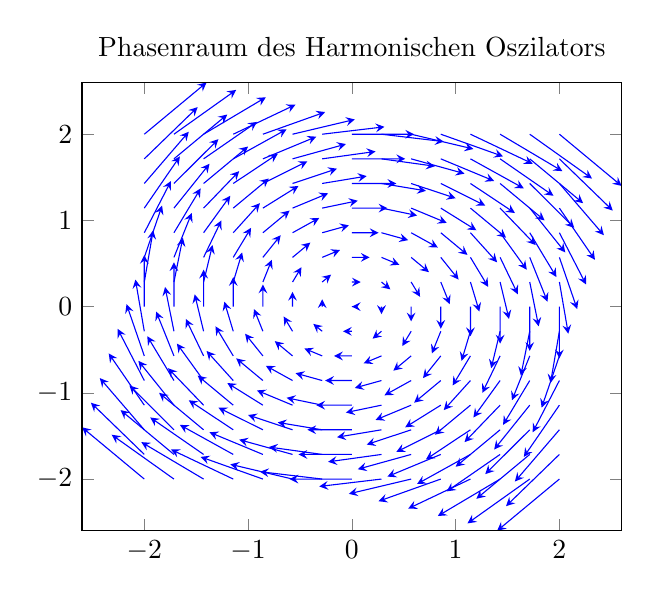
\begin{tikzpicture}
\begin{axis}[title={Phasenraum des Harmonischen Oszilators},domain=-2:2,view={0}{90},axis background/.style={fill=white}]
\addplot3[blue,quiver={u={y},v={-x},scale arrows=0.3},-stealth,samples=15] {y-x};
\end{axis}
\end{tikzpicture}
\item Freier Fall mit Luftwiederstand
\label{sec-2-3-9-1-4}
Aufgabe: Bestime zeitliche Entwicklung von $v$ wenn Körper im Schwerefeld losgelassen wird. $F_R = -cv^2$ \\
      Problem $1-dim$: x wachse nach unten, Start bei $t = 0, x = 0, \dot{x} = 0$
\[F=m\ddot x \Rightarrow m g - c \dot{x}^2 = m\ddot x \Rightarrow \begin{cases} m g - cv^2 &= m \dot{v} \\ v &= \dot{x} \end{cases}\]
Erste Gleichung enthält kein $x$ und kann unabhängig gelöst werden:
\begin{align}
\frac{\d v}{\d t} &= g - \frac{c}{m}v^2 \\
\d t &= \frac{\d v}{g - \frac{c}{m}v^2}
\end{align}
Konstanten und Dimensionen
\[[g] = \si{\meter\per\second\squared};[\frac{c}{m}] = \si{\newton\per\kilo\gram\per\meter\squared\second\squared}\]
Kann leicht Konstanten der Dimension Zeit und Geschwindigkeit bilden:
\[\hat{t} = \sqrt{\frac{m}{g c}},\hat{v} = \sqrt{\frac{g m}{c}}\]
Benutze jetzt die dimensionslosen Variablen $t' = \frac{t}{\hat{t}},v'=\frac{v}{\hat{v}}$
\[\Rightarrow \d t' = \frac{d v'}{1 - v^{2\prime}} = \frac{\d v'}{2}(\frac{1}{1 + v'} + \frac{1}{1 - v'})\]
\[2t' = \ln{1 + v'} - \ln{1 - v'} + c\]
$v' = 0$ bei $t' = 0 \Rightarrow c = 0$
Auflösen nach $v'$: \[e^{2t'} = \frac{1 + v'}{1 - v'} \Rightarrow \ldots\]
\[\Rightarrow v' = 1 - \frac{2}{e^{2t'} + 1} \Rightarrow v = \hat{v}(1 - \frac{2}{e^{\frac{2t}{\hat{t}}}} + 1)\]
$\Rightarrow$ $\hat{v}$ ist Grenzgeschwindigkeit, wird exponentiell angenommen, wenn $t \gg \hat{t}$ \\

Zugabe: einfache physikalische Argumente für die Größe von $c$:
\begin{enumerate}
\item $[c] = \si{\kilo\gram\per\meter}$, Input: $A$ (Querschnitt), $\rho_L$
         $\Rightarrow c \sim \rho_L A$
\item Energiebilanz an verdrängter Luft: \[F_R\cdot l \sim E_{\text{kin,Luft}}\sim\rho_L l A \frac{v^2}{2}\]
\end{enumerate}
\end{enumerate}
\end{enumerate}
% Emacs 25.1.1 (Org mode 8.2.10)
\end{document}